\documentclass{article}
\usepackage[utf8]{inputenc}
\usepackage{graphicx}
\usepackage{xcolor}


\title{Documentation}
\author{Liza Dahiya}
\date{May 2020}

\begin{document}

\maketitle

\section{Week 1}
\subsection{Star Clusters}
Stars are born in cluster (groups of many thousands/million stars). Two distinct types of star cluster can be distinguished: \textbf{globular clusters} are tight groups of hundreds of thousands of very old stars, while \textbf{open clusters} generally contain less than a few hundred members, and are often very young. Open clusters become disrupted over time by the gravitational influence of giant molecular clouds as they move through the Galaxy, but cluster members will continue to move in broadly the same direction through space even though they are no longer gravitationally bound; they are then known as a stellar association, sometimes also referred to as a moving group. \par
Star clusters visible to the naked eye include the \textbf{Pleiades} (M45), \textbf{Hyades}, and the \textbf{Beehive Cluster} (M44).
\subsection{Nebulae}
A nebula is a giant cloud of dust and gas in space. Some nebulae (more than one nebula) come from the gas and dust thrown out by the explosion of a dying star, such as a supernova. Other nebulae are regions where new stars are beginning to form. For this reason, some nebulae are called "star nurseries."
\subsubsection{How do stars form in a nebula?}
Nebulae are made of dust and gases—mostly hydrogen and helium. The dust and gases in a nebula are very spread out, but gravity can slowly begin to pull together clumps of dust and gas. As these clumps get bigger and bigger, their gravity gets stronger and stronger.
\par
Eventually, the clump of dust and gas gets so big that it collapses from its own gravity. The collapse causes the material at the center of the cloud to heat up-and this hot core is the beginning of a star.
\subsubsection{Types of Nebulae}
\textbf{Classical types}\\
    Objects named nebulae belong to 4 major groups. Before their nature was understood, galaxies ("spiral nebulae") and star clusters too distant to be resolved as stars were also classified as nebulae, but no longer are.
    \begin{itemize}
        \item H II regions, large diffuse nebulae containing ionized hydrogen.
        \item Planetary nebulae
        \item Supernova remnant (e.g., Crab Nebula)
        \item Dark nebula
        \item Not all cloud-like structures are named nebulae; Herbig–Haro objects are an example. 
    \end{itemize}
\begin{enumerate}
    \item \textbf{Diffuse nebulae}\\
    Most nebulae can be described as diffuse nebulae, which means that they are extended and contain no well-defined boundaries. Diffuse nebulae can be divided into \textbf{emission nebulae, reflection nebulae and dark nebulae}.
    
    \begin{itemize}
        \item Visible light nebulae may be divided into \textbf{emission nebulae}, which emit spectral line radiation from excited or ionized gas (mostly ionized hydrogen); they are often called H II regions, H II referring to ionized hydrogen), and reflection nebulae which are visible primarily due to the light they reflect. Emission nebulae are usually the sites of recent and ongoing star formation.
        \item \textbf{Reflection nebulae} themselves do not emit significant amounts of visible light, but are near stars and reflect light from them. Reflection nebulae are also usually sites of star formation. They are usually blue because the scattering is more efficient for blue light. Reflection nebulae and emission nebulae are often seen together and are sometimes both referred to as diffuse nebulae.
        \item Similar nebulae not illuminated by stars do not exhibit visible radiation, but may be detected as opaque clouds blocking light from luminous objects behind them; they are called \textbf{dark nebulae}. They are physically very similar to reflection nebulae; they look different only because of the geometry of the light source, the cloud and the Earth. Dark nebulae are also often seen in conjunction with reflection and emission nebulae. 
    \end{itemize}
    A typical diffuse nebula is a few hundred light-years across. Although these nebulae have different visibility at optical wavelengths, they are all bright sources of infrared emission, chiefly from dust within the nebulae.
    
    \item \textbf{Planetary nebulae}\\
    Planetary nebulae are the remnants of the final stages of stellar evolution for lower-mass stars. Evolved asymptotic giant branch stars expel their outer layers outwards due to strong stellar winds, thus forming gaseous shells, while leaving behind the star's core in the form of a white dwarf. 
    
    Radiation from the hot white dwarf excites the expelled gases, producing emission nebulae with spectra similar to those of emission nebulae found in star formation regions. They are H II regions, because mostly hydrogen is ionized, but planetary are denser and more compact than nebulae found in star formation regions.
    
    Planetary nebulae were given their name by the first astronomical observers who were initially unable to distinguish them from planets, and who tended to confuse them with planets, which were of more interest to them. Our Sun is expected to spawn a planetary nebula about 12 billion years after its formation.
    
    \item \textbf{Supernova remnants}\\
    A supernova occurs when a high-mass star reaches the end of its life. When nuclear fusion in the core of the star stops, the star collapses. The gas falling inward either rebounds or gets so strongly heated that it expands outwards from the core, thus causing the star to explode.
    
    The expanding shell of gas forms a supernova remnant, a special diffuse nebula. Although much of the optical and X-ray emission from supernova remnants originates from ionized gas, a great amount of the radio emission is a form of non-thermal emission called synchrotron emission. This emission originates from high-velocity electrons oscillating within magnetic fields.
\end{enumerate}
\subsection{Galaxies}
Galaxies are sprawling systems of dust, gas, dark matter, and anywhere from a million to a trillion stars that are held together by gravity. Nearly all large galaxies are thought to also contain supermassive black holes at their centers. In our own galaxy, the Milky Way, the sun is just one of about 100 to 400 billion stars that spin around Sagittarius A*, a supermassive black hole that contains as much mass as four million suns.
\\
The deeper we look into the cosmos, the more galaxies we see. One 2016 study estimated that the observable universe contains two trillion—or two million million—galaxies. Some of those distant systems are similar to our own Milky Way galaxy, while others are quite different.
\subsubsection{Types of Galaxies}
\begin{enumerate}
    \item \textbf{Spiral Galaxies}\\
    More than two-thirds of all observed galaxies are spiral galaxies. A spiral galaxy has a flat, spinning disk with a central bulge surrounded by spiral arms. That spinning motion, at speeds of hundreds of kilometers a second, may cause matter in the disk to take on a distinctive spiral shape, like a cosmic pinwheel. Our Milky Way, like other spiral galaxies, has a linear, starry bar at its center.
    \item \textbf{Elliptical galaxies} are shaped as their name suggests: They are generally round but can stretch longer along one axis than along the other, so much so that some take on a cigar-like appearance. The universe's largest-known galaxies—giant elliptical galaxies—can contain up to a trillion stars and span two million light-years across. Elliptical galaxies may also be small, in which case they are called dwarf elliptical galaxies.
    
    Elliptical galaxies contain many older stars, but little dust and other interstellar matter. Their stars orbit the galactic center, like those in the disks of spiral galaxies, but they do so in more random directions. Few new stars are known to form in elliptical galaxies. They are common in galaxy clusters.
    
    \item \textbf{Lenticular galaxies}, such as the iconic Sombrero Galaxy, sit between elliptical and spiral galaxies. They're called “lenticular” because they resemble lenses: Like spiral galaxies, they have a thin, rotating disk of stars and a central bulge, but they don't have spiral arms. Like elliptical galaxies, they have little dust and interstellar matter, and they seem to form more often in densely populated regions of space.
    \item \textbf{Irregular Galaxies}\\
    Galaxies that are not spiral, lenticular, or elliptical are called irregular galaxies. Irregular galaxies—such as the Large and Small Magellanic Clouds that flank our Milky Way—appear misshapen and lack a distinct form, often because they are within the gravitational influence of other galaxies close by. They are full of gas and dust, which makes them great nurseries for forming new stars.
\end{enumerate}

\subsubsection{Galactic Clusters and Mergers}
Some galaxies occur alone or in pairs, but they are more often parts of larger associations known as groups, clusters, and superclusters. Our Milky Way, for instance, is in the Local Group, a galaxy group about 10 million light-years across that also includes the Andromeda galaxy and its satellites. The Local Group and its neighbor galaxy cluster, the Virgo Cluster, both lie within the larger Virgo Supercluster, a concentration of galaxies that stretches about 100 million light-years across. The Virgo Supercluster, in turn, is a limb of Laniakea, an even bigger supercluster of 100,000 galaxies that astronomers defined in 2014. \par
\vspace{0.2em}
Galaxies in clusters often interact and even merge together in a dynamic cosmic dance of interacting gravity. When two galaxies collide and intermingle, gases can flow towards the galactic center, which can trigger phenomena like rapid star formation. Our own Milky Way will merge with the Andromeda galaxy in about 4.5 billion years.
\begin{itemize}
    \item Clusters change very slowly (it takes almost as long as the age of the Universe for significant changes to occur in clusters), thus clusters retain an imprint of how they were formed. This makes them a good probe of the history of structure and galaxy formation.
    \item Clusters tend to hold onto the gas in their systems, unlike galaxies, where the gas is forced out through supernova explosions. In other words, clusters are closed systems. By studying the chemical composition of clusters, it is possible to get a history of nucleosynthesis in the Universe.
    \item The force of gravity that holds clusters together comes mostly from dark matter, making clusters an excellent way to study dark matter in the Universe.






\end{itemize}
\subsubsection{Galactic Origins}
The universe's first stars ignited some 180 million years after the big bang, the explosive moment 13.8 billion years ago that marks the origins of the universe as we know it. Gravity had sculpted the first galaxies into shape by the time the universe turned 400 million years old, or less than 3 percent of its current age.

Astronomers now think that nearly all galaxies—with possible exceptions—are embedded in huge haloes of dark matter. Theoretical models also suggest that in the early universe, vast tendrils of dark matter provided normal matter the gravitational scaffold it needed to coalesce into the first galaxies.

But there are still open questions about how galaxies form. Some believe that galaxies formed from smaller clusters of about one million stars, known as globular clusters, while others hold that galaxies formed first, and later birthed globular clusters. It's also difficult to figure out how many of a given galaxy's stars formed in situ from its own gas, versus forming in another galaxy and joining the party later.
\subsection{Binary Stars}
More than four-fifths of the single points of light we observe in the night sky are actually two or more stars orbiting together. The most common of the multiple star systems are binary stars, systems of only two stars together. These pairs come in an array of configurations that help scientists to classify stars, and could have impacts on the development of life. Some people even think that the sun is part of a binary system.
\par
\textbf{Binary stars} are two stars orbiting a common center of mass. The brighter star is officially classified as the primary star, while the dimmer of the two is the secondary (classified as A and B respectively). In cases where the stars are of equal brightness, the designation given by the discoverer is respected.
\subsubsection{Types of binaries}
Binary pairs can be classified based on their orbit.
\begin{enumerate}
    \item \textbf{Wide binaries} are stars that have orbits that keep them spread apart from one another. These stars evolve separately, with very little impact from their companions. They may have once contained a third star, which booted the distant companion outward while eventually having been ejected themselves.
    
    \item \textbf{Close binaries}, on the other hand, evolve nearby, able to transfer their mass from one to the other. The primaries of some close binaries consume the material from their companion, sometimes exerting a gravitational force strong enough to pull the smaller star in completely.
\end{enumerate}
The pairs can also be classified based on how they are observed, a system that has overlapping categories.
\begin{enumerate}
    \item \textbf{Visual binaries} are two stars with a wide enough separation that both can be viewed through a telescope, or even with a pair of binoculars. Five to 10 percent of visible stars are visual binaries.
    \item \textbf{Spectroscopic binaries} appear close even when viewed through a telescope. Scientists must measure the wavelengths of the light the stars emit and determine their binary nature based on features of those measurements.
    \item \textbf{Eclipsing binaries} are two stars whose orbits are at an angle so that, from Earth, one passes in front of the other, causing an eclipse. This feature is based on the line of sight rather than any particular feature of the pair.
    \item \textbf{Astrometric binaries} are stars that seem to dance around an empty space; that is, their companions cannot be identified but only inferred. Such a companion may be too dim to be seen, or could be hidden in the glare from the primary star.
\end{enumerate}
\subsubsection{Discovery and evolution}
The first binary stars seen were visual binaries. In 1617, at the request of a fellow scientist, Galileo Galilei turned his telescope toward the second star from the end of the handle of the Big Dipper, discovering that one star seemed to be two; ultimately it turned out to be six. In 1802, Sir William Herschel, who cataloged about 700 pairs of stars, first used the term "binary" in reference to these double stars.
\\ \par
Stars travel around the galaxy, and sometimes a massive star captures a passing one, creating a new binary pair. But this is a rare event. More commonly, the envelope of gas and dust that collapses in on itself to form a star splits and forms two or more stars instead. These stars evolve together, though not necessarily identically.
\\ \par
How a pair of stars evolve depends on their distance from each other. Wide binaries have very little effect on each other, and so they often evolve much like single stars. Close binaries, however, impact each other's evolution, with mass transfers changing the composition of the stars. If one star in a close binary system explodes in a supernova or sheds its outer layers and forms a pulsar, often the companion is destroyed. If it survives, it continues to orbit the newly formed body, perhaps passing on more of its material.
\\ \par
Binary star systems provide the best means for scientists to determine the mass of a star. As the pair pulls on each other, astronomers can calculate the size, and from there determine characteristics such as temperature and radius. These factors help characterize single main sequence stars in the universe.
\\ \par
The closest star system to Earth — Alpha Centauri — includes a binary pair of stars, Alpha Centauri A and Alpha Centauri B. The third star, Proxima Centauri, is roughly one-fifth of a light-year away (roughly 13,000 sun-Earth distances; some astronomers debate whether Proxima Centauri should be considered part of the same system.) While no stars in the habitable zone have been found in the binary star part of Alpha Centauri, the planet Proxima Centauri b was announced in 2016 in the habitable region of its star. However, scientists are divided as to whether a red dwarf star such as Proxima Centauri has stable enough "space weather" to prevent radiation or heat surges diminishing the chance for life on a nearby planet.
\subsubsection{Is the sun a binary star?}
In the 1980s, scientists suggested the presence of \textbf{Nemesis}, a second star — either a brown dwarf, dim red dwarf or white dwarf — in the sun's system as a reason behind the periodic mass extinctions that occurred in Earth's history, which some paleontologists suggest have occurred in 26-million-year cycles, though the cyclical nature is under debate.
\\ \par
In 2017, a study showed that almost every star like the sun likely had a companion when they were born. A survey using the Very Large Array in New Mexico and the James Clerk Maxwell Telescope in Hawaii examined dozens of systems and found that the younger ones generally had a wide separation, and the older ones had a narrow separation. 
\\ \par
Modeling suggested that most stars would form with a distance between them, and then either move closer together or drift apart, breaking gravitational bonds. In the case of the sun, it's still unclear if Nemesis did exist. If it had, the sun's sibling likely moved away billions of years ago.
\\ \par
Some scientists suggest that there is evidence out there for a Nemesis. Evidence they cite includes the distant orbit of dwarf planet Sedna, the well-defined edge of the Kuiper Belt (a debris disk in our solar system), and the orbits of objects in the Oort Cloud (icy rocks beyond Pluto's orbit). 
\\ \par
Separately, there are research teams pursuing the track of a purported "Planet Nine" ice giant planet that is at the edge of our solar system. In 2016, Konstantin Batygin and Mike Brown (both researchers at the California Institute of Technology) stated that Planet Nine may be altering the orbits of objects in the Kuiper Belt.

\subsection{Types of Brightness}
\begin{enumerate}
    \item \textbf{Visual Brightness}\\
    The word magnitude in astronomy, unless stated otherwise, usually refers to a celestial object’s apparent brightness or apparent \textbf{visual magnitude}. The intrinsic brightness of stars, on the other hand, is called luminosity or absolute magnitude. For the remainder of this post, we’ll be using the word magnitude to talk about a star’s apparent visual magnitude. \par
    
    The apparent magnitude of an object only tells us how bright an object appears from Earth. It does not tell us how bright the object is compared to other objects in the universe. For example, from Earth the planet Venus appears brighter than any star in the sky. However, Venus is really much less bright than stars, it is just very close to us. Conversely, an object that appears very faint from Earth, may actually be very bright, but very far away. 
    
    \item \textbf{Surface Brightness}\\
    In astronomy, surface brightness quantifies the \textbf{apparent brightness} or \textbf{flux density per unit angular area} of a spatially extended object such as a galaxy or nebula, or of the night sky background. An object's surface brightness depends on its surface luminosity density, i.e., its luminosity emitted per unit surface area. In visible and infrared astronomy, surface brightness is often quoted on a magnitude scale, in magnitudes per square arc second in a particular filter band or photometric system.
\end{enumerate}
\subsubsection{Formulas}
The brightness $B$ is the amount of light that we detect from an object. It can mathematically be represented as luminosity $L$ distributed equally over its Area: 
$$B=\frac{L}{4 \pi D^2}$$
But usually the brightness of astronomical objects is measured in \textbf{magnitudes}, which is given by $m$ as:
$$m_1-m_2=-2.5 log_e (\frac{B_{star1}}{B_{star2}})$$
where if lets say the LHS term comes out be 1 we can say that Star 1 is 2.5 times brighter than Star 2. \\
The surface brightness, $S$ is given by, the visual area is given by A:
$$S=m+2.5 log_{10} A$$

\subsubsection{Limited Magnitude}
In astronomy, \textbf{limiting magnitude} is the faintest apparent magnitude of a celestial body that is detectable or detected by a given instrument.\par
In some cases, limiting magnitude refers to the upper threshold of detection. In more formal uses, limiting magnitude is specified along with the strength of the signal (e.g., "10th magnitude at 20 sigma"). Sometimes limiting magnitude is qualified by the purpose of the instrument (e.g., "10th magnitude for photometry") This statement recognizes that a photometric detector can detect light far fainter than it can reliably measure.
\section{Week 2}
\subsection{Equatorial Coordinate System}
\textbf{Right ascension} (abbreviated RA; symbol $\alpha$) is the angular distance of a particular point measured eastward along the celestial equator from the Sun at the March equinox to the (hour circle of the) point in question above the earth. Right ascension is the celestial equivalent of \textbf{terrestrial longitude}. \\
\\
In astronomy, \textbf{declination} (abbreviated dec; symbol $\delta$) is one of the two angles that locate a point on the celestial sphere in the equatorial coordinate system, the other being hour angle. Declination's angle is measured north or south of the celestial equator, along the hour circle passing through the point in question. Declination in astronomy is comparable to geographic latitude, projected onto the celestial sphere, and hour angle is likewise comparable to longitude.
\begin{center}
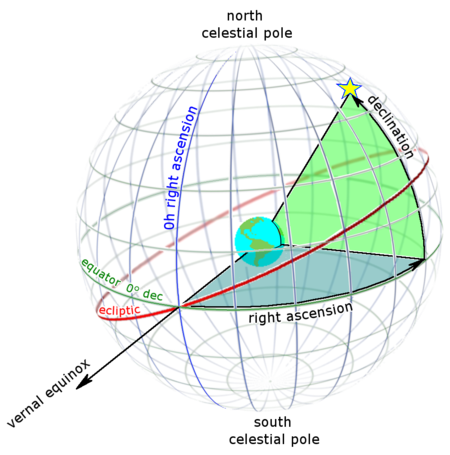
\includegraphics[scale = 0.35]{rc and dec.png}
\end{center}
\section{Week 3}
\textbf{\large Paper on various source detection algorithm approaches for astronomical images}
\subsection{Difficulties}
Difficulties which we face while dealing with astronomical images:
\begin{enumerate}
    \item Many astronomical objects do not show clear boundaries since their intensities are similar to the detection levels and they are mixed with the noise component.
    \item Especially in the case of wide-field deep images showing multiple sources, the sizes and intensities of the different objects present in the images can vary considerably.
\end{enumerate}
Therefore, the main challenge in astronomical object detection
is to separate those pixels that belong to astronomical bodies from
those that belong to background or noise. This task is also referred to as \textbf{object segmentation}. \\
Astronomical detection is usually the first step in the process of building astronomical catalogues. And this process of building an entire catalogue is \textbf{source extraction}.
\subsection{Classification method} 
It is based on two main steps: image transformation and detection criterion. 
\begin{enumerate}
    \item The first one consists in applying changes to the astronomical images to prepare them for the further processing,
    \item the second one consists in classifying pixels that belong to sources and separating them from the background pixels, or in finding those pixels where the sources are centred. 
\end{enumerate}

\subsection{Image Transformation/ Pre-processing}
In astronomical imaging, the objectives of image transformation are, for instance, to filter the noise, to estimate the background or to highlight the objects. Within this image transformation group we find techniques such
as filtering, deconvolution, transforms or morphological operations.
\subsubsection{Basic Image Transformation}
Simple filtering techniques such as median or average are used by many authors. They consist of a sliding window centred on a pixel that computes one of the statistics mentioned for all the pixels in the window, and finally replaces the central pixel by the computed value.

\section{Week 4}
\textbf{\large Hopping Stars Code Documentation}\\

{\color{blue}{main()}} is the main function that drives the code. It takes input until no further input is given i.e. when the user wants to give no more input, they need to leave a blank space when asked for flag input.
\\

In each loop of input it first creates a Point object with the name click and coordinates of click as the input x and input y, then calls a function {\color{blue}list\_stars()} to return a pandas data frame of only those stars that lie within the limiting square with click Point as the center.
Since, a lot of other information is stored along with the star it is good to return the data frame rather than some list containing only the stars coordinates.
\\

While returning such a list we also need to see that if we are returning all the brightest stars closer to the object; well this can be incorporated like if there are a lot of stars within the limiting square then only take the brightest (lets say) 50 stars and remove the other unnecessary faint stars.
\\

After this, we call the function {\color{blue}save\_hops()} to save the hops which would then call a function {\color{blue}min\_distance()} inside it, where {\color{blue}min\_distance()} would return the star which is at the minimum distance from the clicked point. In {\color{blue}min\_distance()} function we first need to create a list of Point object for the stars in the star catalogue with their ra values as x and with dec values as y, which can be used to give back the minimum distanced star. Here, we also take care of two exceptions which are if there is one star found inside the limiting square, which could happen if the user accidentally clicks at a boundary point {\color{red}IndexError} would be raised in such a case. And, other exception could be if there are more than two stars inside the limiting square at same minimum distance, this time an {\color{red}AssertionError} is raised. 
\\

Finally {\color{blue}save\_hops()} returns the latest hop and it gets appended in the hop data frame in the {\color{blue}{main()}} function.
\\

Initially I thought of including a way to check if the editor clicked on the star itself to reduce computation but then on observing closely, I found that the Time complexity of the algorithm is O(n) and wouldn't be affected on introducing new checking method. 
\\

\textbf{Note:} Limiting star is the star with the center as the clicked point and its length being 2*limiting\_value of the length which can be decided as per conditions.

\subsection{Explanation of examples}
\begin{enumerate}
\item x = 200 and y = 20 \\
The Point lies on star 'b' which is returned.
\item x = 100 and y = 10 \\
The Point lies on star 'a' which is returned.
\item x = 0 and y = 0 \\
In this case a square with boundary points as (50, 50), (50, -50), (-50, 50) and (-50, -50) is created and we can see clearly that no star lies inside the limiting square and hence None value is returned.
\item x = 225 and y = 50 \\
In this case a square with boundary points as (275, 100), (275, 0), (175, 100) and (175, 0) is created and we can see clearly that only (200, 20) lies inside the limiting square and hence is returned.
\end{enumerate}


\textbf{Note:} The Nan value can be removed finally if we want by a simple operation.
\end{document}
